\documentclass[a4paper,11pt]{article}

\usepackage[utf8]{inputenc}
\usepackage[T1]{fontenc}
\usepackage{mathptmx}

\usepackage[a4paper,text={160mm,220mm},centering]{geometry}

\usepackage{hyperref}
\usepackage{listings}
\usepackage{graphicx}
\usepackage[table]{xcolor}

\lstset{basicstyle={\ttfamily}}

\begin{document}


\unitlength=1mm
\begin{picture}(0,0)(0,10)
\put(-20,25){
\includegraphics[width=0.3\textwidth]{../images/Logo_Bpifrance.png}
  
\includegraphics[width=0.1\textwidth]{../images/Logo-France-2030-rouge-bleu.png}}
\end{picture}

\begin{center}

{  \Huge\bfseries
  Projet Décysif --- Livrable 2.1 }

{  \Large\bfseries
Constitution d’une base de fichiers d’entrée
représentatifs des difficultés rencontrées pour la
preuve automatique.}


\bigskip
\bigskip


\large Yannick Moy (AdaCore), Guillaume Cluzel (TrustInSoft), Matteo
Manighetti (Inria), Claude Marché (Inria)


\end{center}


Ce livrable est constituée d'une base de tests qui se trouve dans le dépot
\href{https://github.com/Decysif/benchmarks}{'benchmarks'} du projet Décysif.

Objectifs du livrable :

\begin{itemize}
\item Repérer les faiblesses du prouveur Alt-Ergo
\item Repérer les problèmes de traduction (ou repérer des problèmes au niveau de l'écriture des théories, par exemple le modèle mémoire de J3) pour tous les prouveurs cvc5, CVC4, Z3, Alt-Ergo.
\end{itemize}

% Une section par répertoire d'exemples avec une description du contenu
% et de la méthodologie des statisques adoptée. Et le résultat de ces statisques
% au démarrage du projet.

% Mettre les statistiques qu'on a quand elles existent.

\section{Exemples issus de Why3}

\subsection{Jeu d'exemples de programmes écrits en WhyML}

Le sous-répertoire \url{why3_examples} contient le jeu d'exemples
extrait du bench complet de Why3, formé de code source dans le langage
WhyML. La documentation de référence est dans le fichier \url{README.md} de ce répertoire.
Pour installer et configurer ce jeu de tests, la commande
\begin{lstlisting}
> ./import_suite.sh
\end{lstlisting}
doit être exécutée au préalable. Ceci récupère une version de
référence de Why3 (1er mars 2024) et compile les commandes nécessaires. Ensuite la commande
\begin{lstlisting}
> ./run_bench.sh
\end{lstlisting}
pour être lancée pour executer les tests proprement dit. Les prouveurs
utilisés pour ces tests sont indiqués dans le fichier
\url{run_bench.sh} lui-même.

Une exécution de référence de ces tests a été lancée le 15 avril 2024
sur le serveur de calcul «~moloch~» de l'équipe Inria Toccata. Ce
serveur dispose de 16 c{\oe}urs «~Intel(R) Xeon(R) CPU E5-2450 v2 @
2.50GHz~» et de 64 Go de memoire centrale. Pour ces tests, 8 c{\oe}urs
ont été utilisés. Sur chaque fichier source, on demande à Why3 de
générer l'obligation de preuve de chaque fonction, de découper la
formule générée en plusieurs sous-formules, puis on appelle un jeu de
prouveur sur chacune des sous-formules. Un temps limite de 5 secondes est donné à chaque exécution de prouveurs. Pour l'exécution de référence,
les prouveurs Alt-Ergo 2.5.2, CVC4 1.8, cvc5 1.0.5 et Z3 4.12.2 ont
été utilisés. Les résultats sont enregistrés dans des fichiers de
session de preuve de Why3, pouvant donner lieu à diverses
statistiques. Voici des statistiques globales pour l'exécution de
référence, le nombre total d'obligation de preuve est de 41389:
\begin{center}
  \rowcolors{2}{gray!25}{white}
  \begin{tabular}{|l|r|r|r|r|r|}
    \hline
  \rowcolor{gray!50} Prouveur
  & \multicolumn{1}{p{0.13\textwidth}|}{nombre de buts}
  & \multicolumn{1}{p{0.13\textwidth}|}{nombre de buts prouvés}
  & \multicolumn{1}{p{0.13\textwidth}|}{temps minimal}
  & \multicolumn{1}{p{0.13\textwidth}|}{temps maximal}
  & \multicolumn{1}{p{0.13\textwidth}|}{temps moyen}
  \\
  Alt-Ergo 2.5.2                & 41389 & 32170 &  0.00  & 4.98 &  0.12 \\
  CVC4 1.8                      & 41389 & 33650 &  0.01  & 4.81 &  0.17 \\
  cvc5 1.0.5                    & 41389 & 32904 &  0.01  & 4.92 &  0.17 \\
    Z3 4.12.2                     & 41389 & 30713 &  0.01  & 4.96 &  0.07 \\
    \hline
\end{tabular}
\end{center}

\begin{figure}
  \centering
  \hspace*{-0.1\textwidth}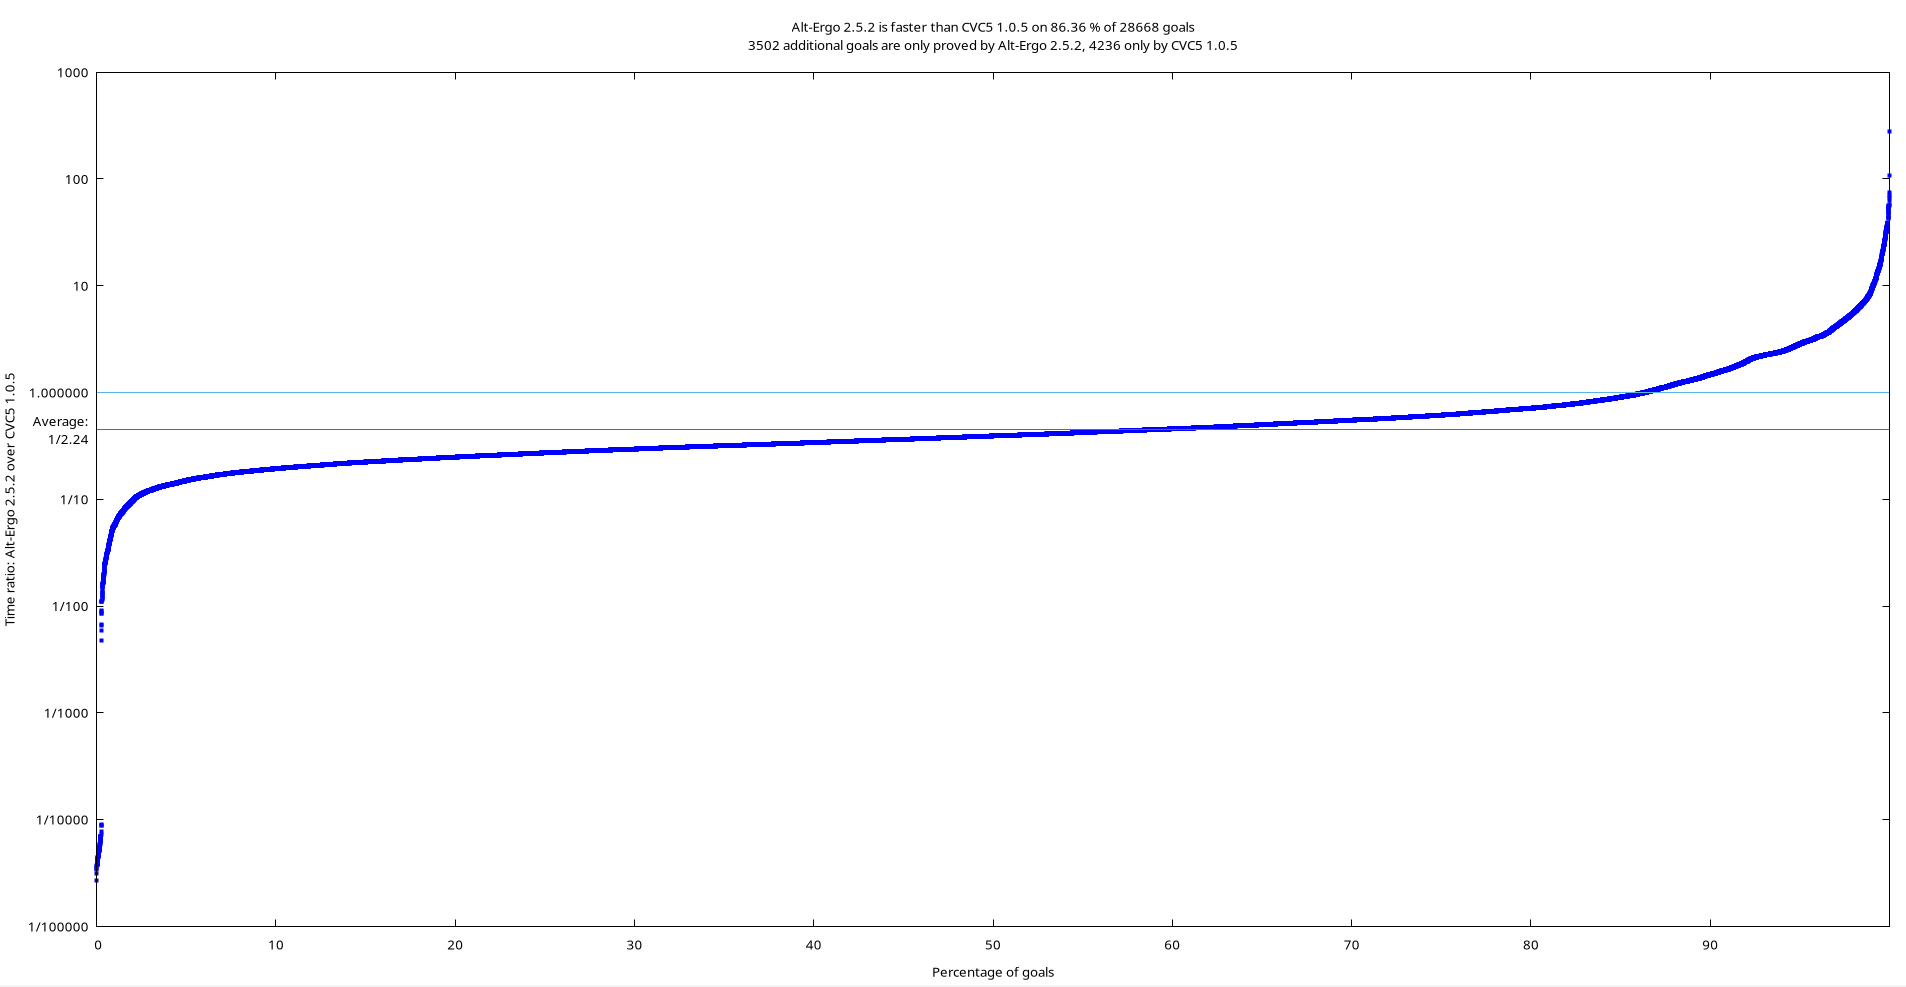
\includegraphics[width=1.2\textwidth]{AE-vs-CVC5.png}
  \caption{Comparaison d'Alt-Ergo et cvc5. Globalement, cvc5 prouve
    plus de buts qu'Alt-Ergo, mais Alt-Ergo est plus rapide. On
    indique aussi que 3502 buts sont prouvés par Alt-Ergo mais pas par
    cvc5, alors que 4236 sont prouvés par cvc5 mais pas par Alt-Ergo.}
  \label{fig:AEvsCVC5}
  \hrulefill
\end{figure}

Des statistiques plus fines peuvent être calculées à la demande sur
les fichiers de sessions. Par exemple, la figure~\ref{fig:AEvsCVC5}
une représentation graphique qui compare les performances de Alt-Ergo
et de cvc5 sur le jeu de test.

En fin de projet, une exécution similaire des outils améliorés seront
rejoués sur les même exemples, et on évaluera les améliorations
apportées en terme de pourcentage de preuve automatique réussies.

\subsection{Exemples écrits spécifiquement pour le projet Décysif}

Le répertoire \url{why3_handcrafted} contient un nombre réduits
d'exemples, qui ont été écrits en WhyML pour spécifiquement tester les
capacités de preuve automatiques des prouveurs. Ces exemples sont
sélectionnés comme représentatifs des difficultés que l'on cherche à
résoudre. L'idéal sera qu'en fin de projet, tous les exemples en
question soient prouvés automatiquement.

\section{Exemples issus de J3}

TODO [Guillaume]

Méthodologie pour extraire des statistique à décrire:
* Nombre de buts prouvés/Nombre de buts au total
TODO: Fixer la version d'alt-ergo

\section{Exemples issus de SPARK}

\subsection{Jeu d'exemples de programmes écrits en SPARK et extraits vers WhyML}

Le sous-répertoire \url{spark_examples} contient le jeu d'exemples extrait du
bench d'exemples de la distribution de SPARK, formé de code source dans le
langage SPARK. La documentation de référence est dans le fichier
\url{README.md} de ce répertoire.

Le code archivé correspond au code Why3 extrait du code SPARK par l'exécution
de gnatprove. Pour installer et configurer ce jeu de tests, les commandes
\begin{lstlisting}
> unzip spark_sexp.zip
> export PATH=$PWD/../why3_examples/why3-88dc033/bin:$PATH
> ./build_environment.sh
> make
\end{lstlisting}
doivent être exécutées au préalable. Cela suppose que le setup dans \url{why3_examples}
a été effectué au préalable afin de récupèrer une version de
référence de Why3 (1er mars 2024) et de compiler les commandes nécessaires. Ensuite la commande
\begin{lstlisting}
> ./run_bench.sh
\end{lstlisting}
doit être lancée pour exécuter les tests proprement dit. Les prouveurs
utilisés pour ces tests sont indiqués dans le fichier
\url{run_bench.sh} lui-même.

Une exécution de référence de ces tests a été lancée le 11 juin 2024
sur le serveur de calcul «~moloch~» de l'équipe Inria Toccata. Ce
serveur dispose de 16 c{\oe}urs «~Intel(R) Xeon(R) CPU E5-2450 v2 @
2.50GHz~» et de 64 Go de memoire centrale. Pour ces tests, 8 c{\oe}urs
ont été utilisés. Sur chaque fichier source, on demande à Why3 de
générer l'obligation de preuve de chaque fonction, de découper la
formule générée en plusieurs sous-formules, puis on appelle un jeu de
prouveur sur chacune des sous-formules. Un temps limite de 5 secondes est donné à chaque exécution de prouveurs. Pour l'exécution de référence,
les prouveurs Alt-Ergo 2.4.0, cvc5 1.0.5 et Z3 4.12.4 ont
été utilisés, avec les drivers propres à GNATprove.
Les résultats sont enregistrés dans des fichiers de
session de preuve de Why3, pouvant donner lieu à diverses
statistiques. Voici des statistiques globales pour l'exécution de
référence, le nombre total d'obligation de preuve est de 135036:
\begin{center}
  \rowcolors{2}{gray!25}{white}
  \begin{tabular}{|l|r|r|r|r|r|}
    \hline
  \rowcolor{gray!50} Prouveur
  & \multicolumn{1}{p{0.13\textwidth}|}{nombre de buts}
  & \multicolumn{1}{p{0.13\textwidth}|}{nombre de buts prouvés}
  & \multicolumn{1}{p{0.13\textwidth}|}{temps minimal}
  & \multicolumn{1}{p{0.13\textwidth}|}{temps maximal}
  & \multicolumn{1}{p{0.13\textwidth}|}{temps moyen}
  \\
  Alt-Ergo 2.4.0                & 135036 &  98822 &  0.00  & 4.96 &  0.09 \\
  cvc5 1.0.5                    & 135036 & 100560 &  0.01  & 4.98 &  0.11 \\
    Z3 4.12.4                     & 135036 & 101915 &  0.00  & 4.89 &  0.04 \\
\hline
\end{tabular}
\end{center}

\subsection{Jeu d'exemples de VC écrites en SMT-LIB2}

Le sous-répertoire \url{spark_handcrafted} contient le jeu d'exemples de VC
écrites directement au format SMT-LIB2 à partir de VC provenant de la suite de
tests SPARK, représentatives des difficultés observées pour prouver des
propriétés arithmétiques. La documentation de référence est dans le fichier
\url{README.md} de ce répertoire.

Les scripts nécessaires pour comparer les résultats de différents prouveurs sur
ces VC sont disponibles dans le sous-répertoire \url{spark_scripts}. Le détail
des commandes est indiqué dans le fichier \url{README.md}. Les résultats sont
enregistrés dans le sous-répertoire \url{results}.  Pour l'exécution de
référence, les prouveurs Alt-Ergo 2.4.0, cvc5 1.0.5 et Z3 4.12.4 et Colibri
2020.9 ont été utilisés.

\begin{center}
  \rowcolors{2}{gray!25}{white}
  \begin{tabular}{|l|r|r|r|}
    \hline
  \rowcolor{gray!50} Prouveur
  & \multicolumn{1}{p{0.13\textwidth}|}{arithmétique entière (51 VC)}
  & \multicolumn{1}{p{0.13\textwidth}|}{arithmétique de bit-vecteurs (20 VC)}
  & \multicolumn{1}{p{0.13\textwidth}|}{arithmétique mixte entière et bit-vecteurs (8 VC)}
  \\
  Alt-Ergo 2.4.0                &  8 &  0 & 0  \\
  cvc5 1.0.5                    & 38 &  1 & 0 \\
  Z3 4.12.4                     & 43 &  1 & 3 \\
    Colibri 2020.9                & 23 & 11 & 1 \\
    \hline
\end{tabular}
\end{center}

\section{Exemples issus de Creusot}

TODO [Claude]

\section{Travail futur}

Tester Colibri2 sur tous les exemples Why3

Quelles autres statistiques peut-on vouloir?

\end{document}
